\documentclass[11pt,a4paper]{article}
\usepackage[margin=1in]{geometry}
\usepackage{booktabs}
\usepackage{graphicx}
\usepackage{float}
\usepackage{hyperref}
\usepackage{amsmath}
\usepackage{parskip}
\usepackage{longtable}
\title{OCQ Cross-Model Status Report}
\author{Codex Workflow}
\date{April 10, 2026}

\begin{document}
\maketitle

\section{Executive Summary}

This document summarizes the first complete cross-model check of the current
catalog-derived OCQ intervention. The method builds an ontology basis from the
MetaTool catalog and injects a low-rank bias into the pre-RoPE key projection
during inference. The core question was whether the same intervention transfers
across model families on the same tool-selection benchmark.

The result is mixed. On \texttt{Qwen/Qwen2.5-7B}, flat K-bias improves MetaTool
Subtask1 substantially. On \texttt{mistralai/Mistral-7B-v0.3}, the same
intervention consistently hurts performance. The present evidence therefore
supports a narrow Qwen-family single-turn claim, not a model-agnostic one.

\section{Intent and Hypothesis}

The immediate purpose of \texttt{R1} was to falsify the easiest overclaim in
the Phase B story: that catalog-derived K-bias is a generally transferable
steering primitive. The working hypothesis before the run was:

\begin{quote}
A catalog-derived ontology basis, injected as flat K-bias, will improve
single-turn MetaTool tool selection on multiple decoder-only model families at
a moderate alpha range near 0.2--0.35.
\end{quote}

\section{Experimental Setup}

The intervention is
\[
K' = K + \alpha (K B_{\mathrm{ont}}) B_{\mathrm{ont}}^{\top},
\]
where \(B_{\mathrm{ont}}\) is a catalog-derived ontology basis. In the current
cross-model run, the basis was built on \texttt{first1} target layers for
portability and bounded execution.

The benchmark is MetaTool Task2-Subtask1 with top-1 tool selection accuracy as
the metric. Qwen and Mistral were evaluated on the full 995-query set, and
Mistral also had an initial 200-query diagnostic run. Llama-3.1-8B was
requested but blocked by gated Hugging Face access.

\begin{table}[H]
\centering
\begin{tabular}{lrrrr}
\toprule
Model & $r_{\min}$ & $r_{\mathrm{median}}$ & $r_{\max}$ & $n_{\mathrm{skipped}}$ \\
\midrule
Qwen2.5-7B & 25 & 27 & 30 & 0 \\
Mistral-7B-v0.3 & 14 & 15 & 19 & 0 \\
\bottomrule
\end{tabular}
\caption{Basis-build diagnostics for the \texttt{first1} setting.}
\end{table}

\section{Results}

\subsection{Qwen2.5-7B, 995 queries}

\begin{table}[H]
\centering
\begin{tabular}{lrr}
\toprule
Method & Top-1 (\%) & Delta vs.\ baseline (pp) \\
\midrule
\texttt{no\_steer} & 73.57 & 0.00 \\
\texttt{ocq\_bias\_a0.2} & 81.11 & +7.54 \\
\texttt{ocq\_bias\_a0.25} & 78.99 & +5.43 \\
\texttt{ocq\_bias\_a0.3} & \textbf{83.12} & \textbf{+9.55} \\
\texttt{ocq\_bias\_a0.35} & 76.38 & +2.81 \\
\texttt{ocq\_bias\_a0.4} & 68.04 & -5.53 \\
\bottomrule
\end{tabular}
\caption{Qwen MetaTool full sweep.}
\end{table}

The positive signal is real and robust enough to matter. The best alpha remains
in the moderate range and gives nearly ten percentage points of lift over the
baseline. The shape is not monotonic: overly strong bias begins to hurt.

\subsection{Mistral-7B-v0.3, 200 and 995 queries}

\begin{table}[H]
\centering
\begin{tabular}{lrrrr}
\toprule
Method & 200 top-1 (\%) & 200 delta & 995 top-1 (\%) & 995 delta \\
\midrule
\texttt{no\_steer} & 52.00 & 0.00 & 55.98 & 0.00 \\
\texttt{ocq\_bias\_a0.2} & 35.50 & -16.50 & 44.12 & -11.86 \\
\texttt{ocq\_bias\_a0.25} & 33.50 & -18.50 & 40.90 & -15.08 \\
\texttt{ocq\_bias\_a0.3} & 29.00 & -23.00 & 37.89 & -18.09 \\
\texttt{ocq\_bias\_a0.35} & 27.50 & -24.50 & 35.38 & -20.60 \\
\texttt{ocq\_bias\_a0.4} & 24.00 & -28.00 & 32.06 & -23.92 \\
\bottomrule
\end{tabular}
\caption{Mistral bounded and full sweeps.}
\end{table}

The bounded Mistral run already showed a monotone collapse with increasing
alpha, and the full run confirms that pattern. This is not a small mismatch but
a clear negative result.

\begin{figure}[H]
\centering
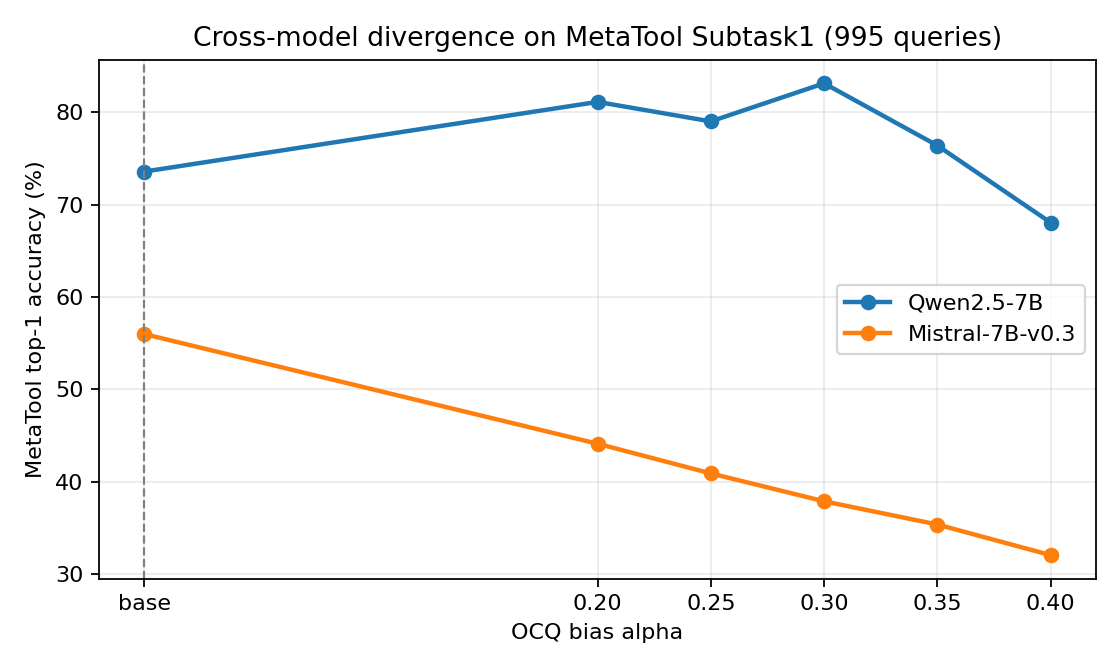
\includegraphics[width=0.86\textwidth]{figures/ocq_cross_model_alpha_sweep_2026_04_10.png}
\caption{Cross-model MetaTool alpha sweep. Qwen shows a moderate-alpha gain,
whereas Mistral degrades monotonically.}
\end{figure}

\section{Interpretation}

The strongest defensible conclusion is narrow:

\begin{quote}
Catalog-derived flat K-bias can improve single-turn tool selection on
Qwen-family models, but it does not currently generalize across model families.
\end{quote}

This result is useful because it falsifies the broad transfer story early.
However, it does not yet explain why Mistral fails. The live hypotheses are
alpha miscalibration, basis mismatch, layer-placement mismatch, or genuine
family-specificity.

\section{Comparison to Prior Steering Lines}

The present method is closest to training-free steering lines such as
SEKA/AdaSEKA, PASTA, and related activation-editing methods, but it differs in
both intervention axis and direction source.

Relative to SEKA/AdaSEKA, this is still a K-side intervention, but the
direction source is a catalog-derived ontology basis rather than task-specific
contrastive SVD experts. Relative to attention-score steering methods such as
PASTA, the present method edits the key-projection subspace itself. The Mistral
failure is therefore especially informative: the mechanism is geometry-sensitive,
not merely a generic increase in tool attention.

\section{What Is Not Yet Supported}

The current evidence does not support multi-turn tool-use claims, facet-gated
superiority, model-agnostic transfer, or production-safe non-tool deployment.
Those claims still need dedicated evidence.

\section{Narrowed Next-Step Plan}

\subsection*{Intent N1}
Keep the strongest defensible claim aligned with the evidence.

\subsection*{Hypothesis}
The viable near-term claim is that flat catalog-derived K-bias improves
single-turn tool selection on Qwen-like models, but its cross-family behavior
is not yet robust.

\subsection*{Verification}
Keep Qwen MetaTool 995 as the positive anchor, keep Mistral MetaTool 995 as the
negative anchor, and do not start multi-turn claims until safety and diagnosis
checks finish.

\subsection*{Intent N2}
Disambiguate the Mistral failure mode.

\subsection*{Hypothesis}
Mistral may fail because the current alpha range is too aggressive rather than
because all ontology directions are invalid.

\subsection*{Verification}
Run a low-alpha sweep with \texttt{no\_steer},
\texttt{ocq\_bias\_a0.05}, \texttt{ocq\_bias\_a0.10},
\texttt{ocq\_bias\_a0.15}, and \texttt{ocq\_bias\_a0.20}. If at least one
alpha reaches \(\ge 3\)pp over baseline, treat the model as recoverable by
calibration; otherwise treat the Mistral result as genuine negative evidence.

\subsection*{Intent N3}
Measure whether the Qwen improvement is compatible with non-tool behavior.

\subsection*{Hypothesis}
If the Qwen gain is useful rather than merely benchmark-specific, the best
MetaTool alpha should preserve MMLU within a modest degradation budget.

\subsection*{Verification}
Run Qwen MMLU subset with \texttt{no\_steer}, \texttt{ocq\_bias\_a0.2}, and
\texttt{ocq\_bias\_a0.3}. If the drop stays within 2pp, the method remains
practically defensible; if the drop exceeds 3--4pp, the result is better framed
as a task-specific tradeoff.

\end{document}
